\documentclass{sig-alternate-05-2015}

\usepackage{float}

% Makes a shortcut for the image folder
\graphicspath{ {./images/} }

\begin{document}


	
% Copyright
\setcopyright{acmcopyright}
%\setcopyright{acmlicensed}
%\setcopyright{rightsretained}
%\setcopyright{usgov}
%\setcopyright{usgovmixed}
%\setcopyright{cagov}
%\setcopyright{cagovmixed}


% DOI
\doi{10.475/123_4}

% ISBN
\isbn{123-4567-24-567/08/06}

\title{Experiment on Performance Difference between Test Driven Development and Code First Test After}

\numberofauthors{3}
\author{
% 1st. author
\alignauthor
	Mads Riisom\\
	\affaddr{University of Southern Denmark}\\
	\affaddr{Odense, Denmark}\\
	\email{marii13@student.sdu.dk}
% 2nd. author
\alignauthor
	Tenna Cortz\\
	\affaddr{University of Southern Denmark}\\
	\affaddr{Slagelse, Denmark}\\
	\email{tecor13@student.sdu.dk}
% 3rd. author
\alignauthor
	Henrik Bolding Frank\
	\affaddr{University of Southern Denmark}\\
	\affaddr{Odense, Denmark}\\
	\email{hefra13@student.sdu.dk}
}

\maketitle
\begin{abstract}
\textit{Background:} Test Driven Development (TDD) is considered a good approach concerning productivity compared to the more common Code First Test After (CFTA) approach, and it works by implementing the tests first, when the tests are done the developer implements just enough logic to pass the test. \textit{Goal:} The group aim to investigate if there is a performance gain in using TDD over CFTA. \textit{Method:} The group performed an experiment using 65 test subjects, who received one of four coding tasks, the tasks had the same end result, but the tasks were described and had to be solved using different approaches with either step by step instructions (Sliced) or free text (Non-sliced) requirement descriptions. Further the subjects had to answer a questionnaire before and after the coding task. \textit{Result:} The experiment showed that with this test group the approach was less important than how detailed the task was described.

\textit{Conclusion:} From this experiment the group cannot make any generalized conclusion as the test group is not a representative of the target group, but there seem to be no real difference between TDD and CFTA.

\end{abstract}


\begin{keywords}
bla bla bla

IN BOLD!

\end{keywords}


\section{Introduction}
Intro intro intro

Something about the test-last and test-first approaches?

\section{Related work}
Related work...
TDD and CTFA
External sources

\section{Research method}
The experiment aimed to investigate the performance difference between TDD and the CFTA approach, with either step by step instructions (Sliced) or free text (Non-sliced). To investigate this the group performed an experiment using third semester Software Engineering bachelor students at SDU as test subjects.

Before and after the experiment was conducted, the students were handed a pre- and a postquestionnaire respectively.
The prequestionnaire contained questions regarding the students perception of their own skill level, where the postquestionnaire contained questions about how well the students thought they had performed during the experiment.

The task the students were to develop were based on four possible tasks that were distributed among the students. They were to develop an application that could calculate the bow\-ling score of a single game, without a graphical user interface. Further the students had to develop a software solution and provide a test environment, that tested the requirements of the task. These requirements for the calculations were explained in the task descriptions, where it were expected for the students to use the specified approach.
The tasks were as follows:
\begin{itemize}
	\item Non-sliced, test-last (NSTL)
	\item Sliced, test last (SLTL)
	\item Non-sliced test first (NSTF)
	\item Sliced, test first (SLTF)
\end{itemize}
The test-last approach tasks were where the students had to implement the requirement, followed by implementing the test which ensures the fulfillment of the requirement.
The test-first approach tasks were where the students had to implement a test to fulfiill the requirement, and then implement as little code to satisfy the test.
The sliced tasks were where the requirements were described step-by-step, whereas the non-sliced tasks had requirement descriptions in one full textblock.


The four tasks were randomly distributed among the students with no knowledge to the group of which students got which specific task. This were decided as the group had previous knowledge of the students strengths and weaknesses, and could therefore insinuate a biased distribution.

While performing the experiment the group participated in a supporting capacity, as well as observers and coordinators. While helping the students with the difficult parts of the experiment, the group gained more insights into the different tasks, and the students' approaches to the tasks. These insights could influence the group's objectivity to the experiment process as well as their perception of the results.

At the beginning of the experiment the students received a code skeleton to work from, to ensure that the solutions would have a similar structure, and therefore would be easier to compare. The submitted solutions was evaluated using an ordinal scale, from where it were decided whether the student were in one of the following three states; failed, critical and passed.

The states are described as follows:
\begin{itemize}
	\item Failed state - Solutions that has no chance to fulfill the requirements
	\item Critical state - Solutions that has a high probability to run, but fulfillment of requirements is questionable
	\item Passed state - Solutions fulfilling the requirements
\end{itemize}

Afterwards the solutions' states and questionnaires were analysed to see if there was a correlation between the test-first or the test-after approach, and the task description's granularity.

\section{Results}
The dataset the experiment is based on, consists of 65 data points, from where 3 data points were rejected as they did not fulfill the requirements of the questionnaires, in other words they were either double or incomplete submission. Therefore, only 62 data points are represented in the following section.

All the subjects had submitted a zip-file containing their solution based on the code skeleton provided for the experiment. The 3 states the submissions were categorized in, were evaluated as if it was a real exam submission.
The states were divided as follows:

\begin{itemize}
	\item 23 - failed state attempts
	\item 16 - critical state attempts
	\item 23 - passed state attempt
\end{itemize}

\begin{figure}[H]
	\centering
	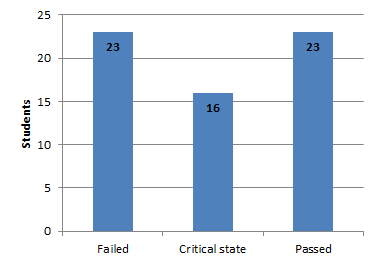
\includegraphics[width=0.4\textwidth]{img01}
	\caption{Distribution of student's performance}
	\label{fig:Distribution of student's performancel}
\end{figure}
% Her er et eksempel på hvordan man laver en ref til en figur. Jeg sætter et label som er en markør og bruger den til at link med, på den måde opdatere tallet hvis der kommer end ny figur ind.
Figure~\ref{fig:Distribution of student's performancel} represents the distribution of student's performance in the experiment, where the evaluation of their submitted code were divided into the three states.\\

As the distribution of the tasks were random, and each student got exactly one task. The number of students receiving the individual tasks were distributed as illustrated in figure~\ref{fig:Task distributions}:

\begin{figure}[H]
	\centering
	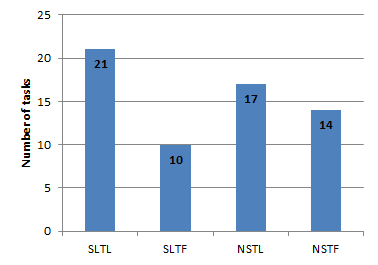
\includegraphics[width=0.4\textwidth]{img02}
	\caption{Task distributions}
	\label{fig:Task distributions}
\end{figure}

38 students used the test-last approach, and 24 students used the test-first approach. Further it is an exceptional case where both the sliced and non-sliced tasks were equally distributed with 31 of each.

After the assessment of the code submissions, it is possible to look at the answers of the questionnaires. Shown in figure~\ref{fig:Student's own experience rating} the student's perception of their own programming experience in these fields; General programming, C{\#}, Visual Studio, Unit testing, NUnit testing framework and Test-driven development (TDD).
The students were rating their experience on the scale: None, Novice, Intermediate and Expert.

\begin{figure}[H]
	\centering
	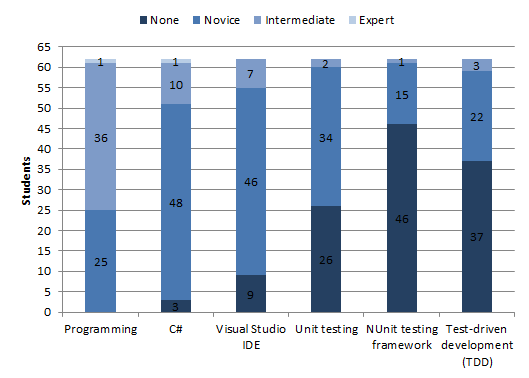
\includegraphics[width=0.4\textwidth]{img03}
	\caption{Student's own experience rating}
	\label{fig:Student's own experience rating}
\end{figure}

It is interesting to see that the students who ended up with TF tasks rated themselves lower in their perception of their experience in TTD.

\begin{figure}[H]
	\centering
	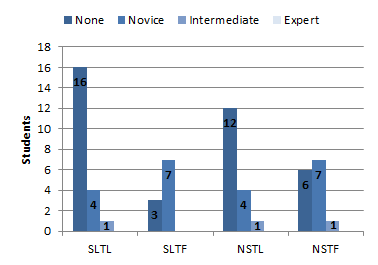
\includegraphics[width=0.4\textwidth]{img04}
	\caption{TDD experience in tasks}
	\label{fig:TDD experience in tasks}
\end{figure}

When looking at figure~\ref{fig:Student's own experience rating} and ~\ref{fig:TDD experience in tasks}, there are more people with none TDD-experience in the test-last approach, which also is an exceptional case.

The experiment aimed to investigate the performance difference between Test-Driven Development (TDD) and the more common Code First Test After (CFTA) approach, with either step by step instructions (Sliced) or free text (Non-sliced).\\

As the experiment aimed to investigate the performance based on the four tasks distributed amongst the students, figure~\ref{fig:Student's task performance} shows the code states divided by the tasks.

\begin{figure}[H]
	\centering
	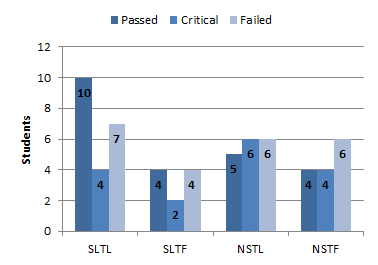
\includegraphics[width=0.4\textwidth]{img05}
	\caption{Student's task performance}
	\label{fig:Student's task performance}
\end{figure}

As it is stated in figure~\ref{fig:Student's task performance}, there are a tendency for the students' submissions to pass with sliced tasks.

Figure~\ref{fig:SLTL percentage distributions with relative task numbers} shows the distributions between the students self-rating of programming experience level (None, Novice, Intermediate, Expert), and their correlating submission state (Passed, Critical, Failed), divided into each of the tasks respectively.
It is important to notice that there were no students who have rated their programming experience  as "None" which means that they could have excluded this in figure~\ref{fig:SLTL percentage distributions with relative task numbers}-\ref{fig:NSTF percentage distributions with relative task numbers}. These are however included in the diagrams as it was an option in the pre-questionnaire, and therefore if excluded, could give a skewed view of the students programming experience levels. This does also apply for the "Expert" ratings which is described show in figure~\ref{fig:SLTL percentage distributions with relative task numbers}.

\begin{figure}[H]
	\centering
	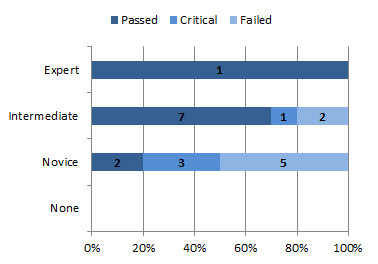
\includegraphics[width=0.4\textwidth]{img06}
	\caption{SLTL percentage distributions with relative task numbers}
	\label{fig:SLTL percentage distributions with relative task numbers}
\end{figure}

Here it is seen that 100\% of all students who rated their programming experience to be "Expert" has submitted a solution that fulfilled the requirements satisfying, where it was only 70\% and 20\% in respectively "Intermediate" and "Novice".
It is important to notice that there were only one student who rated him- or herself as an "Expert" in programming experience, which means that he could have been excluded from the statistical analysis of this task, as the "Expert" percentage are misleading the reader. The rest of the percentages are for the critical submissions 10\% and 30\%, and for the failed submissions 20\% and 50\% respectively for the "Intermediate" and the "Novice" students.

\begin{figure}[H]
	\centering
	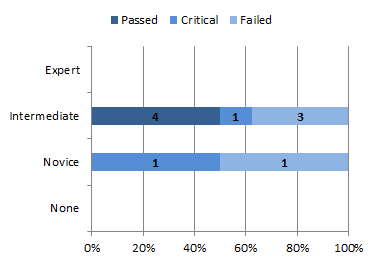
\includegraphics[width=0.4\textwidth]{img07}
	\caption{SLTF percentage distributions with relative task numbers}
	\label{fig:SLTF percentage distributions with relative task numbers}
\end{figure}

In figure~\ref{fig:SLTF percentage distributions with relative task numbers} it is seen that only 50\% of the "Intermediate" students submitted solutions which fulfilled the requirements satisfying, where there are none "Novice" students who did. On the other hand it is seen that it is respectively 12.5\% and 50\% in the "Intermediate" and "Novice" who were in the Critical state. The last percentages are 37.5\% and 50\% for respectively the "Intermediate" and the "Novice" students are those who failed.

\begin{figure}[H]
	\centering
	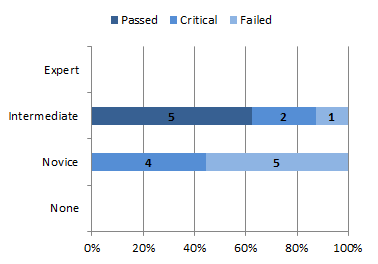
\includegraphics[width=0.4\textwidth]{img08}
	\caption{NSTL percentage distributions with relative task numbers}
	\label{fig:NSTL percentage distributions with relative task numbers}
\end{figure}

Figure~\ref{fig:NSTL percentage distributions with relative task numbers} shows the distribution of the students' experience and states of the NSTL tasks. Here it is also seen that it is only the students who have rated themselves as "Intermediate" experienced in programming, who submitted solutions that fulfilled the requirements with 62.5\%. This means that the "Novice" students had a distribution, with 44.5\% critical and 55.5\% failed submissions. Whereas the "Intermediate" students had 25\% critical and 12.5\% failed solution submissions.

\begin{figure}[H]
	\centering
	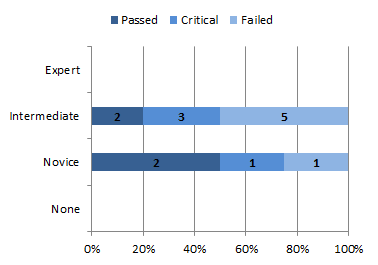
\includegraphics[width=0.4\textwidth]{img09}
	\caption{NSTF percentage distributions with relative task numbers}
	\label{fig:NSTF percentage distributions with relative task numbers}
\end{figure}

Figure~\ref{fig:NSTF percentage distributions with relative task numbers} shows the distribution of the student's experience and states of the NSTF tasks. Here it is seen that both the "Intermediate" and the "Novice" students have submitted solutions that fulfilled the requirements, with a distribution of 20\% and 50\% respectively. Further the critical is distributed 30\% and 25\% where the failed is distributed 50\% and 25\% respectively for the "Intermediate" and the "Novice" students.

Figure~\ref{fig:Total normalized data distributed in tasks} is a visualization of the total normalized data divided into the four different tasks. These data is calculated based on the weights: Passed=1, critical=0.5, failed=0.01.

\begin{figure}[H]
	\centering
	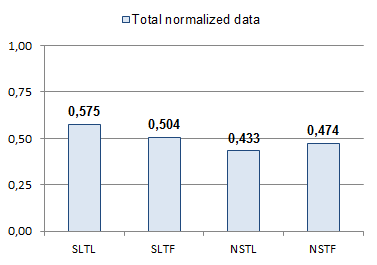
\includegraphics[width=0.4\textwidth]{img10}
	\caption{Total normalized data distributed in tasks}
	\label{fig:Total normalized data distributed in tasks}
\end{figure}

It is seen that the students who had the sliced tasks performed better than the students who had the non-sliced tasks.

Figure~\ref{fig:Novice normalized data distributed in tasks in accordance to total normalized data} shows "Novice" and "Intermediate" normalized data respectively, in accordance to the total normalized data.

\begin{figure}[H]
	\centering
	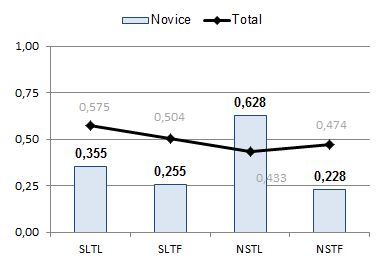
\includegraphics[width=0.4\textwidth]{img11}
	\caption{Novice normalized data distributed in tasks in accordance to total normalized data}
	\label{fig:Novice normalized data distributed in tasks in accordance to total normalized data}
\end{figure}

In figure~\ref{fig:Novice normalized data distributed in tasks in accordance to total normalized data} it is illustrated that the "Novice" normalized data is lower than the total in all tasks but in the NSTL task. This data suggest that people who rate their programming experience as "Novice" is more predisposed to doing well when given the NSTL task, than when given one of the other tasks.

\begin{figure}[H]
	\centering
	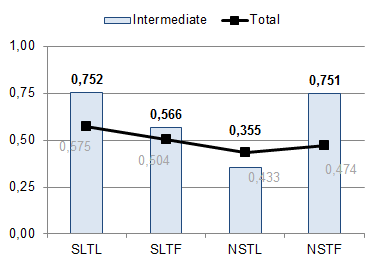
\includegraphics[width=0.4\textwidth]{img12}
	\caption{Intermediate normalized data ditsributed in tasks in accordance to total normalized data}
	\label{fig:Intermediate normalized data ditsributed in tasks in accordance to total normalized data}
\end{figure}

Figure~\ref{fig:Intermediate normalized data ditsributed in tasks in accordance to total normalized data} shows that the "Intermediate" normalized data is higher than the total in all tasks but in the NSTL. Which suggest that people who rates their programming experience at "Intermediate" is more predisposed to do worse when given the NSTL tasks in comparison if given one of the other tasks.

\section{Threats to validity}

The threats to the Internal validity of this experiment are mostly related to the selection process. The experiment was conducted while the students were performing a test, which would indicate that they were highly motivated to perform well.\\

Further External threats to the validity were amongst others the \textit{Interaction of setting and treatment}, as the test subjects were given small simple tasks to complete, which does not represent a real world setting the results from an experiment in the field might vary. \textit{Interaction of history and treatment} is an important factor as the subjects had received lectures in all the topics tested in the experiment a few weeks up to the experiment. The participants were not representative of the target group (Software Developers) which also had an effect on the results, as they were unable to perform at the same level as the level as the target group.\\

One of the major Social threats were the subjects inability to work alone, as some talked together during the experiment, which was not intended. The group did not consider \textit{Hypothesis guessing} a threat for the coding part of the experiment, but had to reevaluate it after the end of the experiment, as the subjects did not have more than 5  weeks of experience with TDD from received lectures. This might have impacted the subjects answers more or less in favor of TDD in the pre and post questionnaires. Another threat to the Social validity comes from the human discomfort from being evaluated, which can have influenced the results.\\

The principal Conclusion validity is affected by the \textit{heterogeneity of the subjects} was rather large, as the test subjects was still only in the start of their university education, so their previously programming ability still played a major role in their programming proficiency which is also concerning the External validity. The conclusion validity is generally strong because of the high \textit{Statistical Power} in having a large group of participants, but the group do not claim that the results can be generalized for the entire software developer population. 

\section{Discussion}

In this section we compare TDD and CFTA according to our results. The result doesn’t give any clear answer to what is best, but the results indicate that for the students as novice developers it was easier to use the code first approach, which could be because they didn’t know how to solve the problem at first, but used trial and error to solve small parts of the assignment step by step to find a solution that seemed to cover the requirements. When the developer does not know how the code will be structured in the end it is difficult to write tests that will cover everything.\\

This has to be compared to the more experienced developers, who knew how they were going to solve the assignment from the requirements. Which allowed them to write the tests according to their initial solution and then use the tests to identify issues they might run into when implementing the logic later on.\\

But as all of the students are new to programming these are only assumptions, and we have to do more research to find a clear answer, as the results will most likely be different with a group of more experienced developers.\\

For the next iteration of this experiment it is paramount that the students are more clearly instructed in what the assignment is, to ensure that they are more focused on performing the experiment in accordance to description, as the validity of the results become questionable when the students differ from the described pattern of the experiment. \\

To ensure that there was no bias in the assignment of tasks the students received tasks randomly, this has the benefit that we as a group were unable to bias the results by handing out the assignments to the students in a way that would increase the probability of favourable result. The downside to this approach is that there was an unequal distribution of students across the different tasks, but with a sample group of this size it was not an issue.

\section{Conclusion And Future Work}
In this study the group performed an experiment to investigate if there was an increase in productivity when the using TDD instead of CFTA. The test subjects were not representative of the target group of software developers so these findings only reflect how TDD and CFTA compare when used by students. 

But the experiment indicates that for students considering themselves as Novices making the tests first yielded worse results than Test Last. The students considering themselves as intermediate the Test first seemed to yield the best results. But these results has to be tested further to make any generalized conclusion as there is no clear trend in the results.

In the future the group would like to perform a similar test on a group which has a closer relation to the actual target group. The group would also investigate if it would be possible to use a metric to determine a subject's programming proficiency objectively instead of using the user's opinion. This will hopefully lead to a more general conclusion regarding the performance differences regarding TDD and CFTA.

\begin{thebibliography}{3}

\bibitem{fucci1}
  D. Fucci, B. Turhan, M. Oivo,
  \emph{On The Effects of Programming and Testing Skills on External Quality and Productivity in a Test-Driven Development Context},
  Oulu, Finland.
  
\bibitem{fucci2}
  D. Fucci, B. Turhan,
  \emph{A Replicated Experiment on the Effectiveness of Test-first Development},
  Oulu, Finland,
  2013.
  
\bibitem{fucci3}
  D. Fucci, B. Turhan, M. Oivo,
  \emph{Impact of Process Conformance on the Effects of Test-driven Development},
  Oulu, Finland,
  2014.

\end{thebibliography}

\section{Acknowledgments}

First of all, the group wants to thank Dr. Marco Kuhrmann for his participation and help in this experiment. Especially for providing the necessary communication with the former of the experiment kit, and the provided tools and data.\\

The group also wants to thank Davide Fucci, Burak Turhan, Markku Oivo from University of Oulu for providing the experiment kit used in this experiment.\\

Thanks to all students of 3. semester Software Engineering 2016 of University of Southern Denmark for participating in this project.

\end{document}
